\documentclass[11pt,a4paper]{article}

\usepackage{a4wide}
\usepackage{polski}

\usepackage[left=2cm,right=2cm,top=2cm,bottom=3cm]{geometry}

\usepackage[utf8]{inputenc} 

\usepackage{amsmath}
\usepackage{graphicx}

\usepackage{float}
\usepackage{relsize}
\usepackage{subcaption}
\usepackage{tabularx}

\usepackage[colorlinks=true, allcolors=blue]{hyperref}

\usepackage[skip=10pt plus1pt, indent=0pt]{parskip}
\usepackage{indentfirst}

\title{Bazy danych 2 \\
Dokumentacja projektu}
\author{Dominika Boguszewska \\
Piotr Lenczewski \\
Michał Machnikowski \\
Jakub Pęk \\
Tomasz Truszkowski}
\date{Semestr 24L}

\begin{document}

\maketitle

\tableofcontents

\newpage

\section{Temat projektu}

Postanowiliśmy stworzyć aplikację służącą szukaniu osób w celu wspólnego uprawiania sportu. Użytkownicy mogą stworzyć wydarzenie, w którym deklarują miejsce, dzień oraz interesujący ich sport. Także mogą zapisać się na wcześniej utworzone wydarzenie po wyszukaniu takich, które ich interesują.

\section{Grupa docelowa aplikacji}

Nasza aplikacja jest skierowana do osób, które są zainteresowanie aktywnością fizyczną i chcą znaleźć towarzyszy do wspólnego uprawiania sportu. A także dla organizatorów wydarzeń sportowych, którzy chcą łatwo znaleźć uczestników do organizowanych wydarzeń.

\section{Wymagania aplikacji}

\subsection{Wymagania funkcjonalne}

\begin{itemize}
    \item Użytkownik może stworzyć konto.
    \item Przy tworzeniu konta wymagane jest ustawienie silnego hasła.
    \item Po utworzeniu konta wysyłany jest email z potwierdzeniem do użytkownika.
    \item Użytkownik może zalogować się na swoje konto.
    \item Użytkownik może ustawić swoje zdjęcie profilowe.
    \item Użytkownik może ustawić opis swojego profilu.
    \item Użytkownik może dodać własne ogłoszenia z parametrami: rodzaj sportu, liczba poszukiwanych osób, miejsce, czas (jednorazowe czy cykliczne), dodatkowy opis.
    \item Użytkownik może wyszukiwać oferty według podanych kryteriów (np. rodzaj sportu, miejsce, czas).
\end{itemize}
 
\subsection{Wymagania niefunkcjonalne}

\begin{itemize}
    \item Aplikacja działa na systemie operacyjnym Linux.
    \item Aplikacja działa na systemie operacyjnym Windows.
    \item Każda strona aplikacji musi się załadować w przeciągu 2 sekund.
    \item Aplikacja powinna wytrzymać X użytkowników bez strat jakości.
    \item Email wysłany do użytkownika po utworzeniu konta musi do niego dojść w przeciągu 10 minut.
\end{itemize}

\section{Model pojęciowy (E-R)}

\begin{figure} [H]
    \centering
    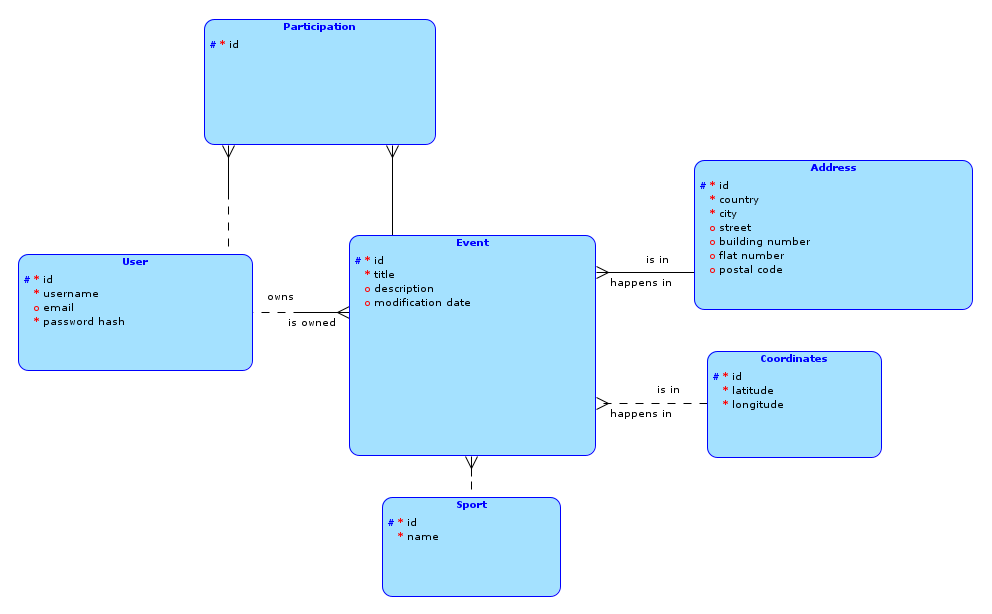
\includegraphics[width=0.95\linewidth]{model/model_er.png}
\end{figure}

\section{Model relacyjny bazy danych}

\begin{figure} [H]
    \centering
    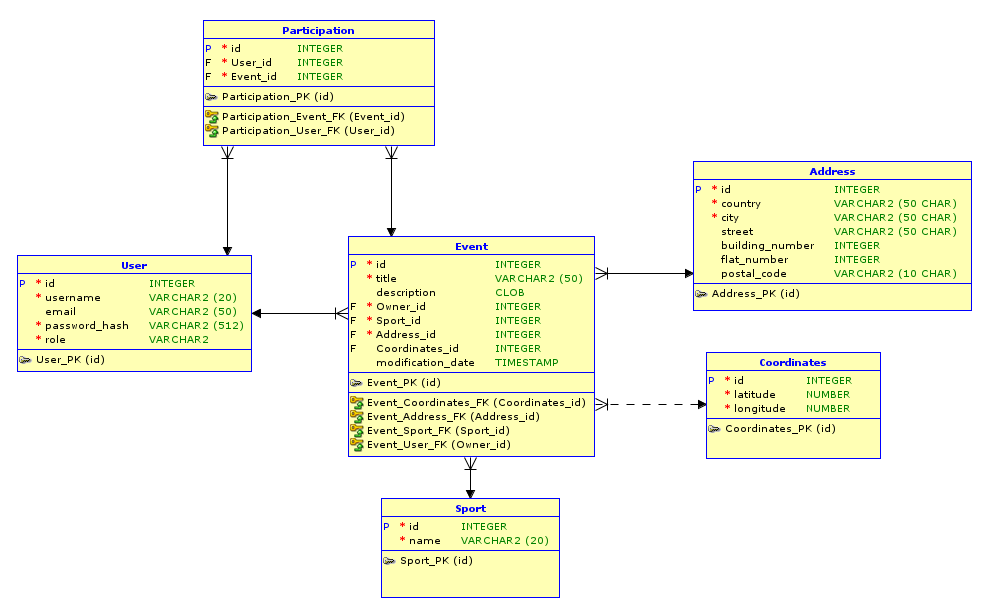
\includegraphics[width=0.95\linewidth]{model/model_rel.png}
\end{figure}

\section{Zdenormalizowany model relacyjny bazy danych}

\begin{figure} [H]
    \centering
    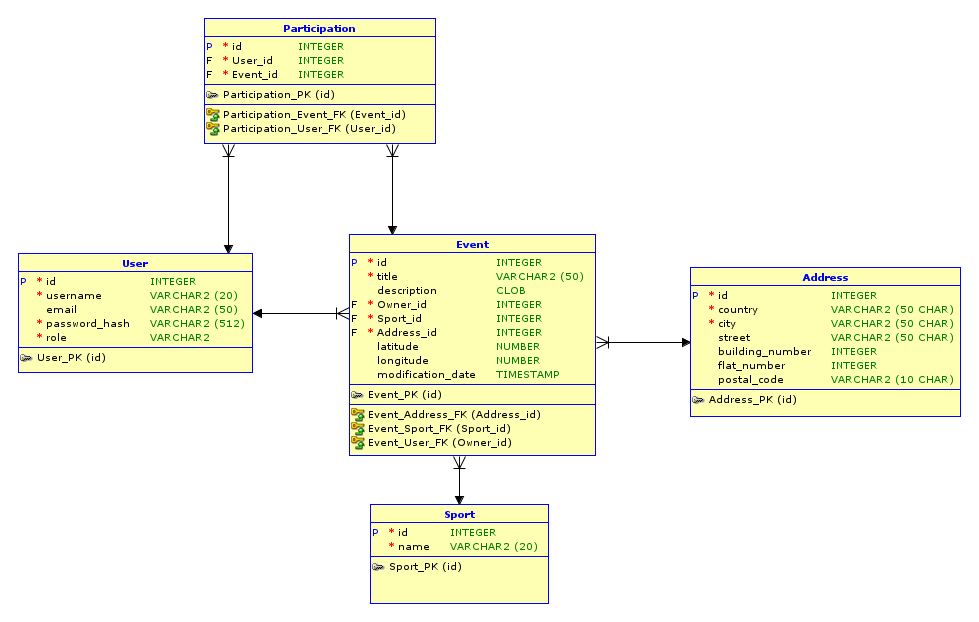
\includegraphics[width=0.95\linewidth]{model/model_denorm.png}
\end{figure}

Podczas procesu denormalizacji usunęliśmy tabelę \textit{Coordinates}, a jej atrybuty \textit{latitude} i \textit{longitude} przenieśliśmy do tabeli \textit{Event}.

\section{Wykorzystane technologie}

\begin{itemize}
    \item MySQL
    \item Java
    \item Spring Boot
    \item Next.js
\end{itemize}

\section{Instrukcja użytkowania}

\subsection{Uruchomienie aplikacji}

Po otworzeniu aplikacji uruchamia się strona powitalna, z której po kliknięciu przycisku \textit{Login} można przejść do formularzy logowania się oraz rejestracji. 

\begin{figure} [H]
    \centering
    
\includegraphics[width=1\linewidth]{pages/welcome.png}
    \caption{Strona powitalna}
\end{figure}

\subsection{Logowanie się i rejestracja}

Następnie użytkownik może zalogować się na już istniejące konto bądź stworzyć nowe. W przypadku rejestracji koniecznie jest podanie silnego hasła, czyli takiego, które składa się z co najmniej 5 znaków w tym co najmniej 1 dużej litery i co najmniej 1 cyfry.

\begin{figure}[H]
    \centering
    \captionsetup{justification=centering,margin=2cm}
        \begin{subfigure}{0.49\textwidth}
            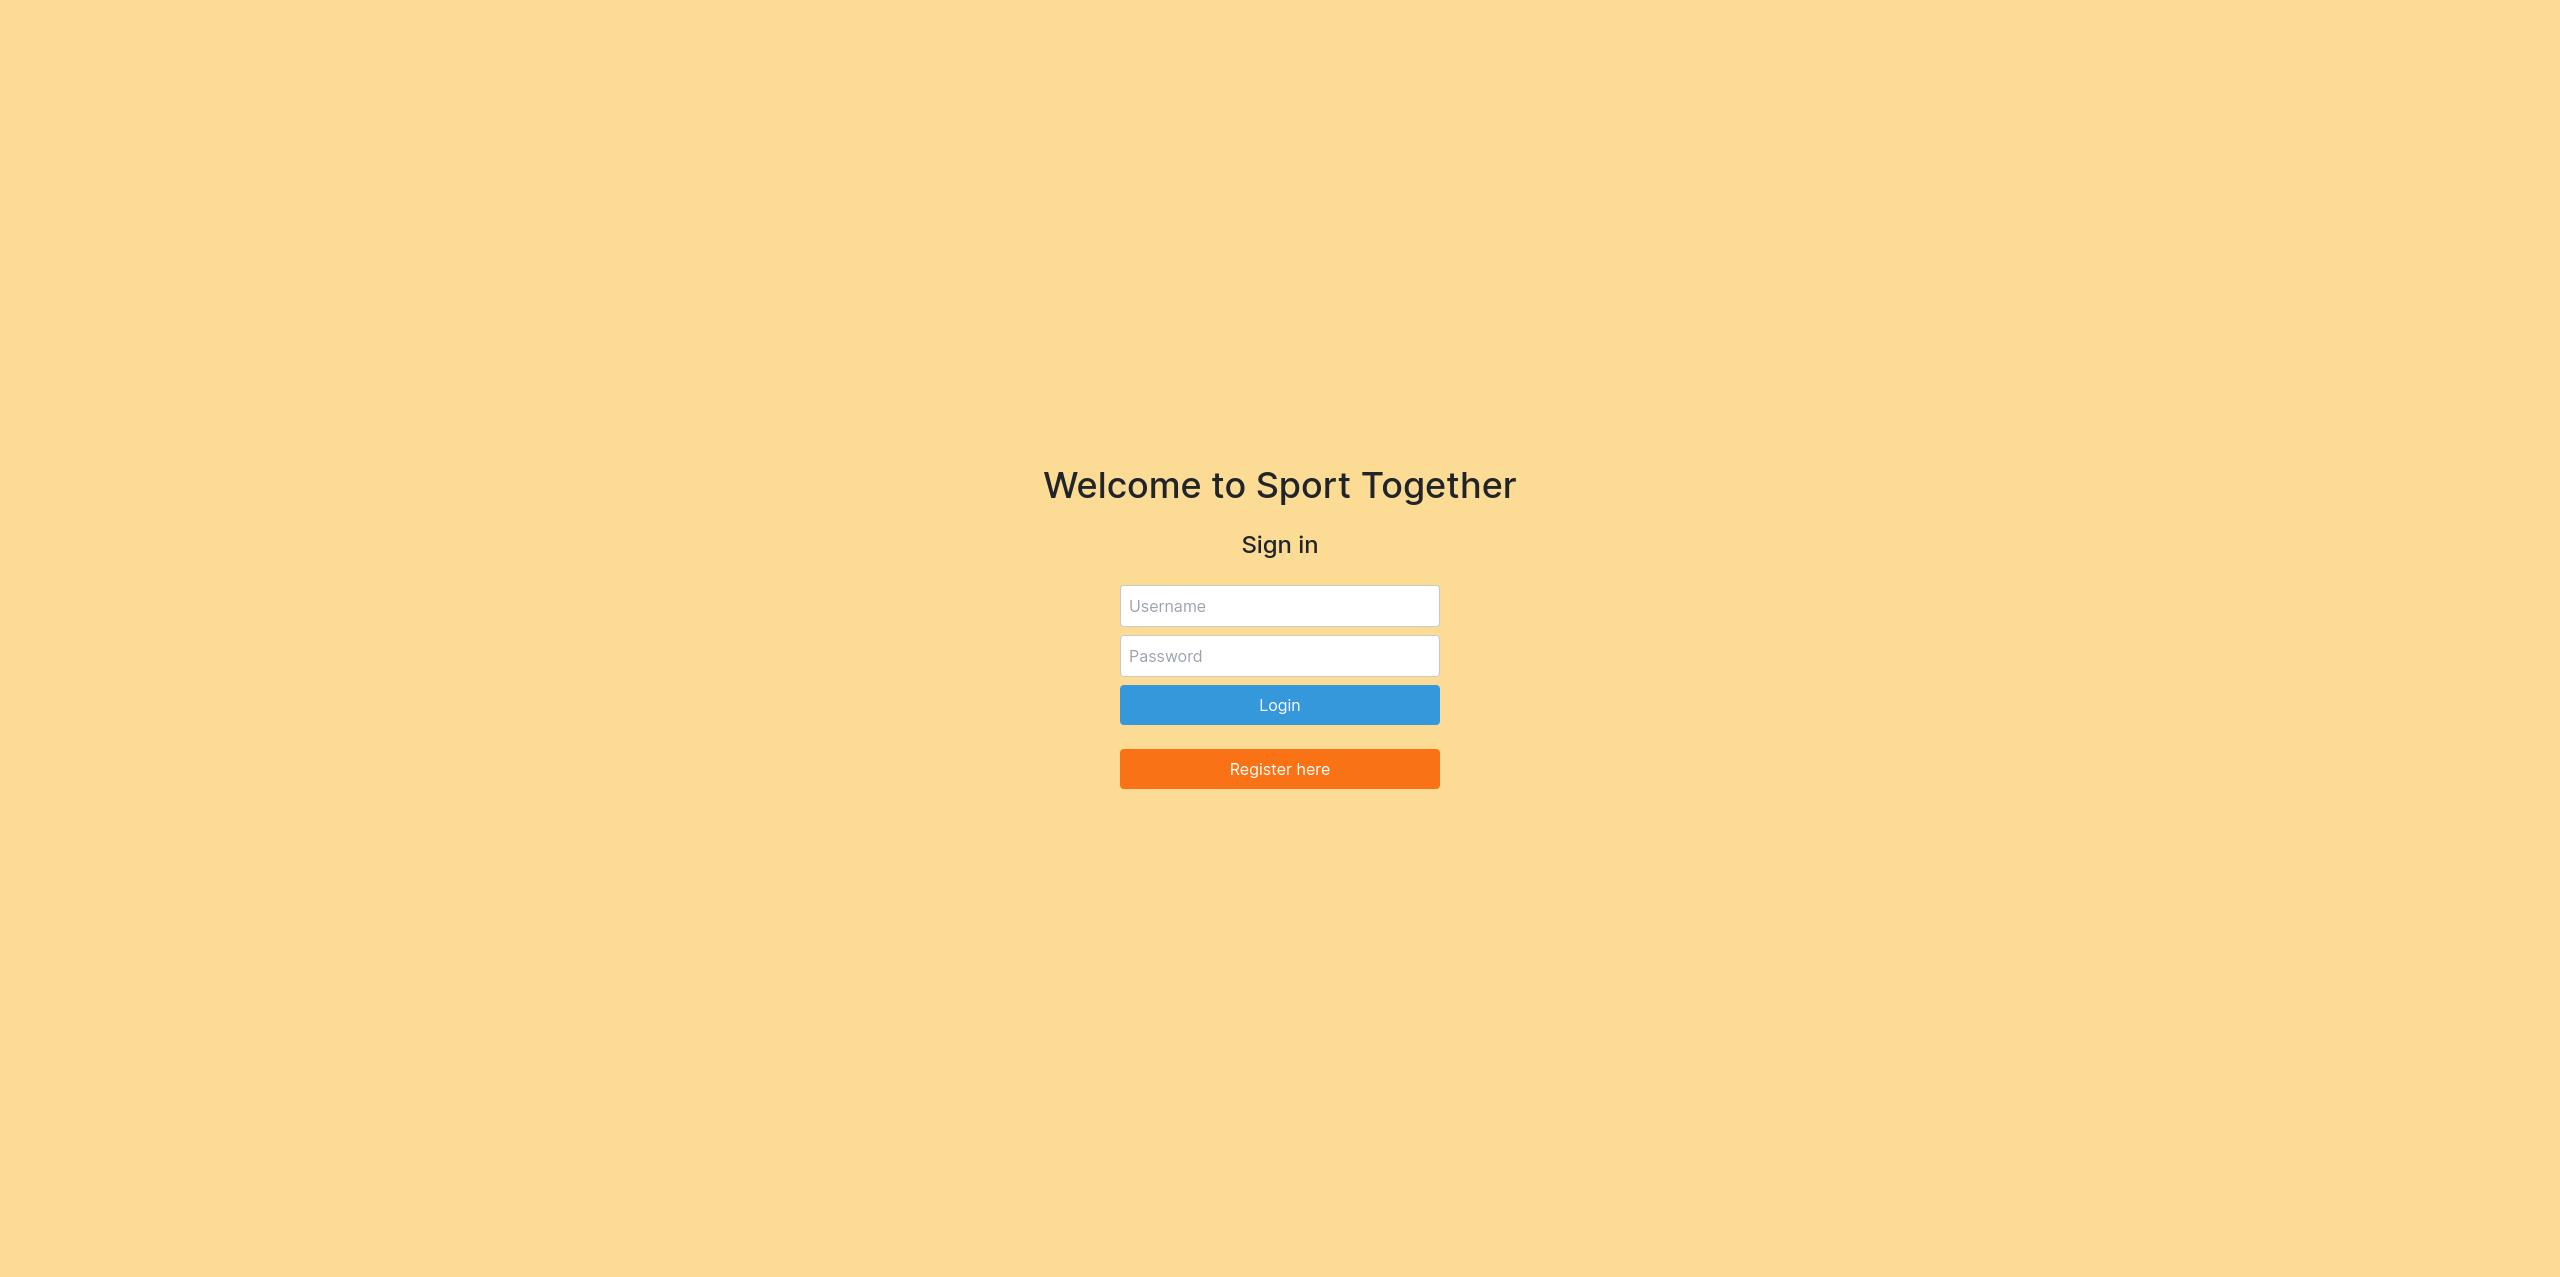
\includegraphics[width=\textwidth]{pages/login_page.png}
            \caption{Formularz logowania się}
        \end{subfigure}
    \hfill
        \begin{subfigure}{0.49\textwidth}
            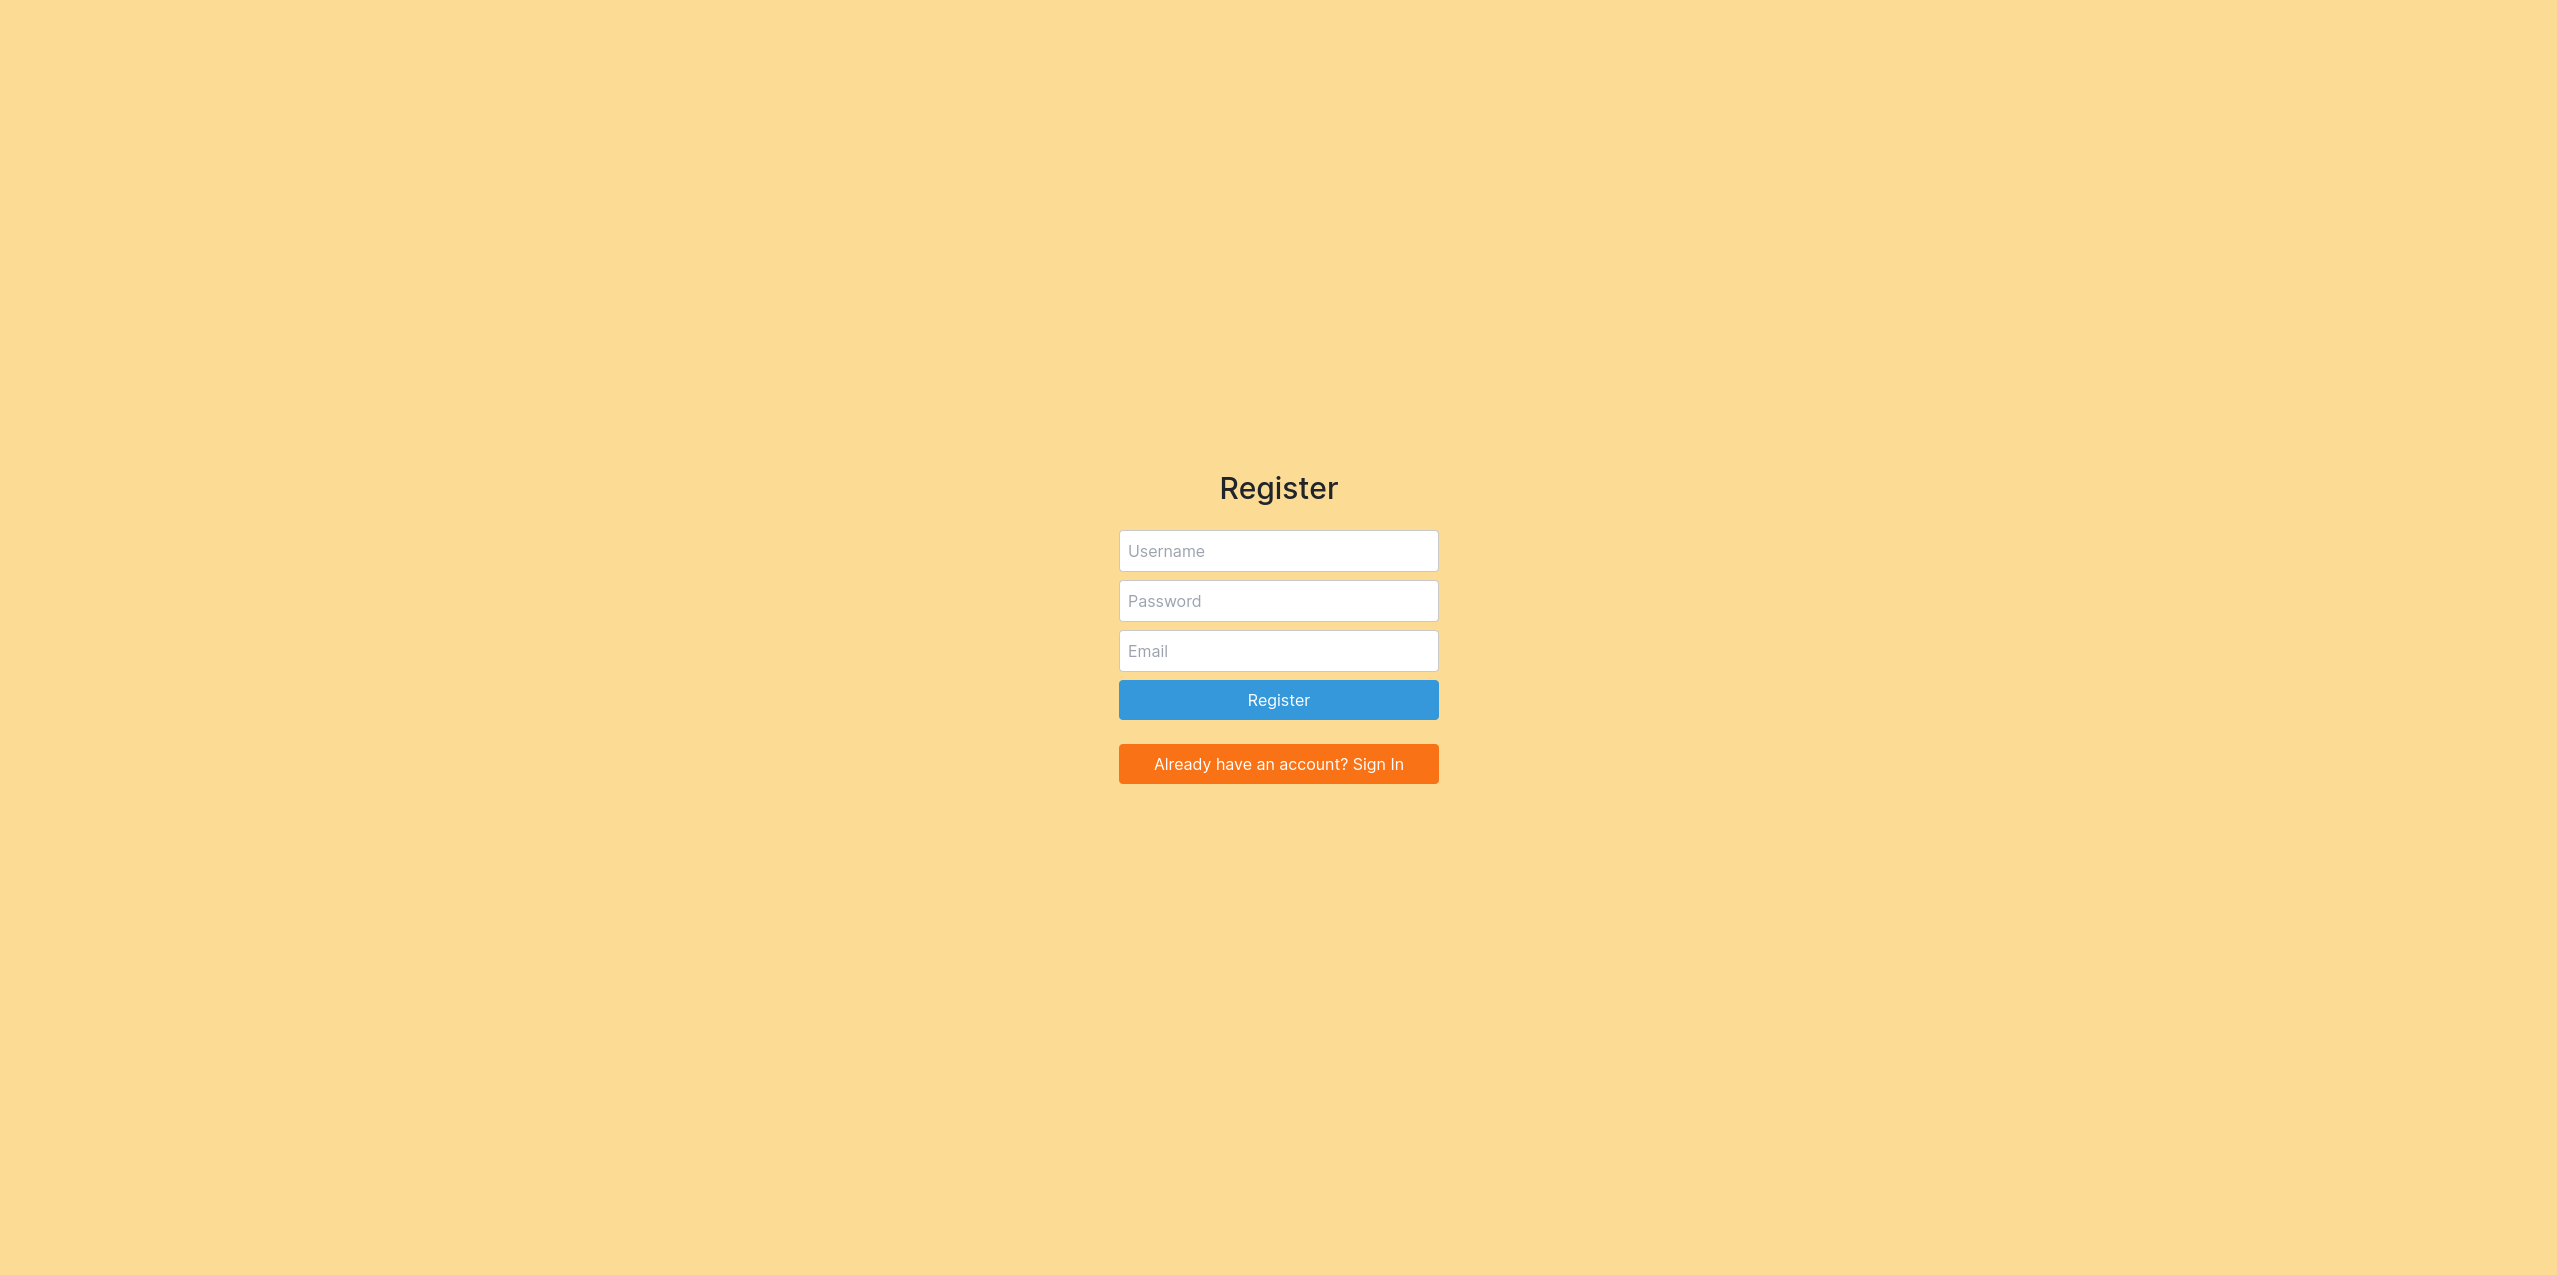
\includegraphics[width=\textwidth]{pages/register.png}
            \caption{Formularz rejestracji}
        \end{subfigure}
\end{figure}

Po tym zostaje przeniesiony na stronę startową, gdzie są wyświetlane wydarzenia, w których uczestniczy oraz te, które organizuje. Może także stamtąd przejść na stronę służącą wyszukiwaniu wydarzeń, wyświetlić informacje o swoim koncie, przejść do formularza tworzenia nowego wydarzenia lub się wylogować.

\begin{figure} [H]
    \centering
    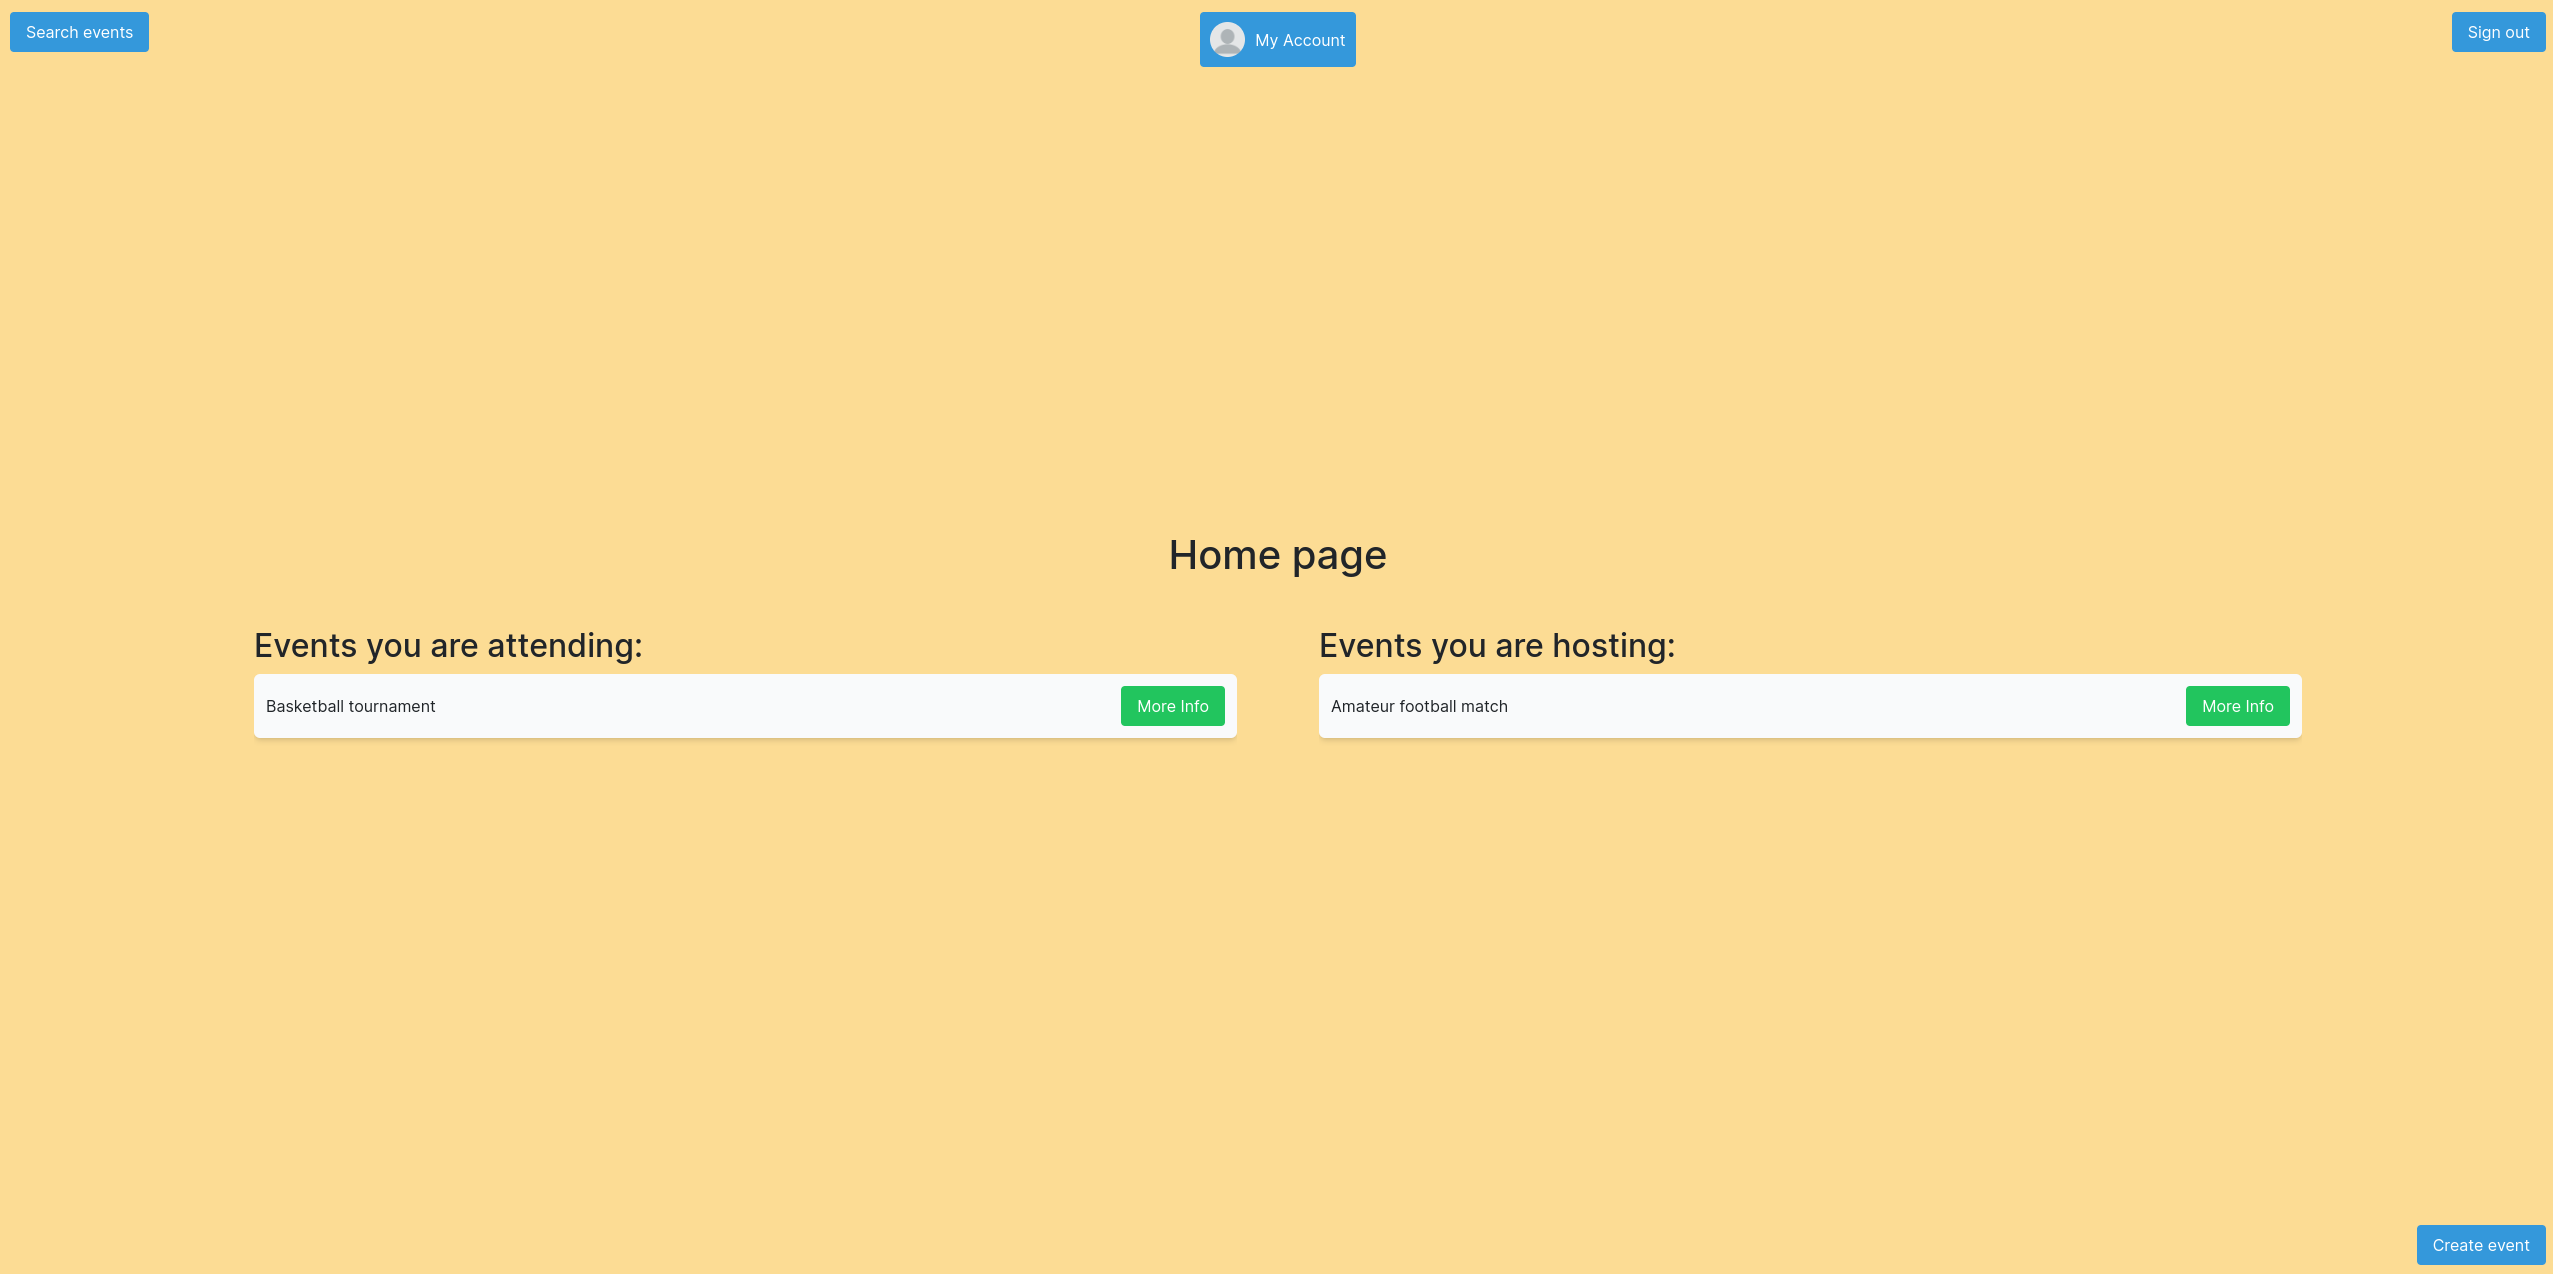
\includegraphics[width=1\linewidth]{pages/home.png}
    \caption{Strona startowa}
\end{figure}

\subsection{Konto użytkownika}

\subsection{Zapisywanie się na wydarzenia}

\subsection{Tworzenie nowych wydarzeń}

\subsection{Wylogowanie się}

\end{document}
